\documentclass{article}
\usepackage{graphicx}
\usepackage{amsmath}
\usepackage{mathtools}
\usepackage{hyperref}
\usepackage{here}
\usepackage{tikz}
\usetikzlibrary{external}
\tikzexternalize % Attiva l'esternalizzazione delle immagini
\usepackage{verbatim}
\usepackage[version=4]{mhchem}
\usepackage{minted}
\usepackage{xcolor}
%\usepackage[version=4]{mhchem}
\usetikzlibrary{shapes.geometric, arrows.meta, positioning}
\usepackage[utf8]{inputenc}
\usepackage{biblatex} %Imports biblatex package
\addbibresource{ref.bib} %Import the bibliography file

\newcommand{\be}{\begin{equation}}
\newcommand{\ee}{\end{equation}}
\newcommand{\ba}{\begin{eqnarray}}
\newcommand{\ea}{\end{eqnarray}}

\title{Conservation Laws}
\author{Simone Cavallero}
\date{July 2024}

\begin{document}

\maketitle

\section{Introduction}
Autocatalytic networks typically involve internal species which make more of themselves and external species which play the role of fuel or waste. While autocatalytic networks lack conservation law, there are still conservation laws for the total mass and conserved fragments of molecules called moieties. These moieties are arranged differently after the reactions so that autocatalytic species manage to make more of themselves. The question we address here is: could these conservation laws for moieties actively rule the production of autocatalytic species? 

\section{Type 1 with fuel and waste}

We start considering the type 1 example with $F$ (fuel) and $W$ (waste) to allow for mass conservation. Using two different fuels for the different reactions, we can write the reactions as:
\begin{equation}
\label{set_reactions}
		\begin{split}
		\ce{\textsf{F}_1 + \textsf{A} & <--> \textsf{B} } \\ 
\ce{\textsf{F}_2 + \textsf{B} & <--> 2 \textsf{A} + \textsf{W}}.	
		\end{split} 
\end{equation}



The stoichiometric matrix is in terms of $F_1$, $F_2$, $W$, $A$ and $B$ :
\begin{center}
    \begin{equation}
        S=\begin{pmatrix}
            -1 & 0 \\
            0 & -1 \\
            0 & 1 \\
            -1 & 2 \\
            1 & -1 \\
        \end{pmatrix}
    \end{equation}
\end{center}

This matrix has a left nullspace of dimension 3, since 3 out of 5 rows are linearly dependent from the other two. A possible basis of the nullspace is then:

\begin{center}
    \begin{equation}
        \Bar{A}=\begin{pmatrix}
            0 \\
            1 \\
            0 \\
            1 \\
            1 \\           
\end{pmatrix} \quad
X=\begin{pmatrix}
            0 \\
            1 \\
            1 \\
            0 \\
            0 \\           
\end{pmatrix} \quad
Y=\begin{pmatrix}
            1 \\
            0 \\
            1 \\
            0 \\
            1 \\           
\end{pmatrix}
    \end{equation}
\end{center}

$\Bar{A}$, $X$, $Y$ can be seen as the moieties that the system is conserving, indeed, written as the following, their value must remain constant throughout the dynamics of the reactions. We find that
\begin{center}
\ba
\Bar{A} &= F_2 + A + B\\
X &= F_2 + W \nonumber \\
Y &= F_1 + W + B \nonumber.
\ea
\end{center}

Based on this, all the species can be expressed as combinations of these moieties:
$A = \Bar{A}, B = \Bar{A}Y, \textsf{F}_1  = Y,
\textsf{F}_2  = \Bar{A} X, W  = XY.$

Reactions \ref{set_reactions} then become, in terms of singular compounds:
\begin{equation}
		\begin{split}
		\ce{\textsf{Y} + \textsf{$\Bar{A}$}& <--> \textsf{$\Bar{A}$Y} } \\ 
\ce{$\Bar{A}$\textsf{X} + \textsf{$\Bar{A}$Y} & <--> 2 \textsf{$\Bar{A}$} + \textsf{XY}}.	
		\end{split} 
\end{equation}

We can identify then, 3 stoichiometric matrices for each of the moieties, taking into account in which reaction they are consumed and produced

\begin{center}
    \begin{equation}
        S_{\Bar{A}}=\begin{pmatrix}
            0 & 0 \\
            0 & -1 \\
            0 & 0 \\
            -1 & 2 \\
            1 & -1 \\
            
\end{pmatrix} \quad
S_{X}=\begin{pmatrix}
            0 & 0 \\
            0 & -1 \\
            0 & 1 \\
            0 & 0 \\
            0 & 0 \\
            
\end{pmatrix} \quad
S_{Y}=\begin{pmatrix}
            -1 & 0 \\
            0 & 0 \\
            0 & 1 \\
            0 & 0 \\
            1 & -1 \\
            
\end{pmatrix}
    \end{equation}
\end{center}

This means that the conservation of the moiety \textcolor{red}{$\Bar{A}$} is hidden in the two reactions 
\begin{equation}
		\begin{split}
  \ce{\textsf{A} & <--> \textsf{B} }	\\
  \ce{\textsf{F}_2 + \textsf{B} & <--> 2 \textsf{A} }
		\end{split} 
\end{equation}

The conservation law for the moiety \textcolor{green}{$X$} is instead hidden in the reaction

\begin{equation}
		\begin{split}
  \ce{\textsf{F}_2 & <--> \textsf{W} }
		\end{split}, 
\end{equation}
whereas for the moiety \textcolor{blue}{$Y$}:
\begin{equation}
		\begin{split}
  \ce{\textsf{F}_1 & <--> \textsf{B} }	\\
  \ce{\textsf{B} & <-->  \textsf{W} }
		\end{split} 
\end{equation}

\begin{figure}
\begin{flushleft}
\begin{minipage}{0.3\textwidth}
\begin{tikzpicture}[>=stealth, thick]
    % Nodes
    \node (A) at (0, 4) {$\Bar{A}$};
    \node (AY) at (3, 4) {$\Bar{A}Y$};
    \node (AX) at (3, 1.25) {$\Bar{A}X$};
    \node (mid) at (3, 2.5) [circle, fill=red, inner sep=1pt] {};
    \node (mid2) at (0.5, 2.9) [circle, fill=red, inner sep=1pt] {};
    
    % Paths
    \draw[->, draw=red] (A) -- (AY);
    \draw[--, draw=red] (AY) -- (mid);
    \draw[--, draw=red ,dash pattern=on 4pt off 4pt] (mid) -- (AX);

    \draw[--, draw=red] (mid) to[out=180, in=-30] (mid2);
    \draw[->, draw=red] (mid2) to[out=90, in=320] (A);
    \draw[->, draw=red] (mid2) to[out=180, in=270] (A);
    
    %\draw[->] (B) to[out=-45, in=135] (A);
    
    % Extra node (dot)
    %\node[circle, fill, inner sep=1pt] at (3, 0) {};
\end{tikzpicture}
\end{minipage}
 \hspace{0.03\textwidth} % Spazio tra le immagini
    % Seconda immagine TikZ
    \begin{minipage}{0.3\textwidth}
    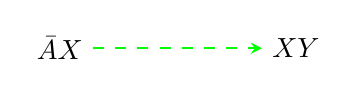
\begin{tikzpicture}[>=stealth, thick]
    % Nodes
    \node (AX) at (0, 2) {$\Bar{A}X$};
    \node (XY) at (3, 2) {$XY$};
    
    % Paths
    \draw[->, draw= green, dash pattern=on 4pt off 4pt] (AX) -- (XY);
    
    
    %\draw[->] (B) to[out=-45, in=135] (A);
    
    % Extra node (dot)
    %\node[circle, fill, inner sep=1pt] at (3, 0) {};
\end{tikzpicture}
    \end{minipage}
    \hspace{0.03\textwidth} % Spazio tra le immagini
    % Seconda immagine TikZ
    \begin{minipage}{0.3\textwidth}
    \begin{tikzpicture}[>=stealth, thick]
    % Nodes
    \node (Y) at (0, 4) {$Y$};
    \node (AY) at (1.5, 2) {$\Bar{A}Y$};
    \node (XY) at (3, 0) {$XY$};
    
    % Paths
    \draw[->, draw=blue ,dash pattern=on 4pt off 4pt] (Y) -- (AY);
    \draw[->, draw=blue ,dash pattern=on 4pt off 4pt] (AY) -- (XY) 
    
    %\draw[->] (B) to[out=-45, in=135] (A);
    
    % Extra node (dot)
    %\node[circle, fill, inner sep=1pt] at (3, 0) {};
\end{tikzpicture}
    \end{minipage}
\end{flushleft}
\caption{Moieties conservations representation. Only moiety \textcolor{red}{$\Bar{A}$} contains an autocatalytic pattern (loop). Moieties \textcolor{green}{$X$} and \textcolor{blue}{$Y$} represents only pure fluxes}
\label{type1}
\end{figure}


 We notice that the autocatalytic behavior of the network (autocatalysis of A) is actually hidden in just one of the the conservation laws, while the others are "fueling" the system to keep the moieties concentration constant.
 Note that just because we are taking the reactions once, when we look at the overall one, we end up with the autocatalysis of A, whereas taking twice the first reaction and once the second, we end up with the autocatalysis of B. This shows that the autocatalytic modes $\mathbf{g}_i$ still play a role to define the autocatalytic behavior.

\section{Type 2 with fuel and waste}

Let's consider now the generic reactions for a type 2 core that allow for mass conservation:

\begin{equation}
\label{set_reactions_2}
		\begin{split}
		\ce{\textsf{F}_1 + \textsf{A} & <--> \textsf{B} } \\ 
\ce{\textsf{F}_2 + \textsf{B} & <--> \textsf{C}} \\
\ce{\textsf{F}_3 + \textsf{C} & <--> \textsf{A} + \textsf{B} + \textsf{W}}
		\end{split} 
\end{equation}

Assuming as rows, respectively species $F_1$, $F_2$, $F_3$, $W$, $A$, $B$ and $C$, the stoichiometric matrix $S$ will appear 

\begin{center}
    \begin{equation}
        S=\begin{pmatrix}
            -1 & 0 & 0 \\
            0 & -1 & 0 \\
            0 & 0 & -1 \\
            0 & 0 & 1 \\
            -1 & 0 & 1 \\
            1 & -1 & 1 \\
            0 & 1 & -1
\end{pmatrix}
\end{equation}
\end{center}

The nullspace has dimension 4, and a possible basis for it can be

\begin{center}
    \begin{equation}
        H=\begin{pmatrix}
            1 \\
            1 \\
            1 \\
            2 \\
            0 \\
            1 \\
            2
\end{pmatrix} \quad
X=\begin{pmatrix}
            1 \\
            0 \\
            0 \\
            0 \\
            0 \\
            1 \\
            1          
\end{pmatrix} \quad
Y=\begin{pmatrix}
            0 \\
            0 \\
            2 \\
            1 \\
            1 \\
            1 \\
            1           
\end{pmatrix} \quad
Z=\begin{pmatrix}
            1 \\
            0 \\
            1 \\
            1 \\
            0 \\
            1 \\
            1
\end{pmatrix}
    \end{equation}
\end{center}

So that the conservation laws for the moieties $H$, $X$, $Y$, $Z$ can be written as

\begin{center}
\ba
H &= F_1 + F_2 + F_3 + 2W + B + 2C\\
         X &= F_1 + B + C\\
          Y &= 2 F_3 + W + A + B + C\\
          Z &= F_2 + W + C
\ea
\end{center}

Based on this, all species must then be combinations of these four moieties:
$A = Y, B = HXY, C = H_2 XYZ, \textsf{F}_1  = HX,
\textsf{F}_2  = HZ, \textsf{F}_3  = H \textrm{Y}_2,
W  = \textrm{H}_2 YZ.$

Reactions \ref{set_reactions_2} then become, in terms of these compounds:

\begin{equation}
\label{cc}
		\begin{split}
		\ce{\textsf{HX} + \textsf{Y} & <--> \textsf{HXY} } \\ 
\ce{\textsf{HZ} + \textsf{HXY} & <--> \textsf{$\textsf{H}_2$XYZ}}	\\
\ce{\textsf{H $\textsf{Y}_2$} +  \textsf{$\textsf{H}_2$XYZ} & <-->  \textsf{Y} + \textsf{HXY} + \textsf{$\textsf{H}_2$YZ}}
		\end{split} 
\end{equation}

The stoichiometric matrix for moiety \textcolor{blue}{H} then, following \ref{cc}, will be

\begin{center}
    \begin{equation}
        S_{H}=\begin{pmatrix}
            -1 & 0 & 0 \\
            0 & -1 & 0 \\
            0 & 0 & -1 \\
            0 & 0 & 2 \\
            0 & 0 & 0 \\
            1 & -1 & 1 \\
            0 & 2 & -1
\end{pmatrix}
    \end{equation}
        \end{center}
Describing the set of reactions

\begin{equation}
		\begin{split}
  \ce{\textsf{F}_1 & <--> \textsf{B} }	\\
  \ce{\textsf{F}_2 + \textsf{B} & <-->  \textsf{C} } \\
  \ce{\textsf{F}_3 + \textsf{C} & <-->  \textsf{B} + \textsf{W} }
		\end{split} 
\end{equation}

These reactions can be shown from the point of view of the moieties through the following graph: \\

\begin{figure}[H]
\begin{center}
\begin{tikzpicture}[>=stealth, thick]
    % Nodes
    \node (HX) at (0, 7) {$HX$};
    \node (Y) at (0, 3.5) {$$};
    \node (HXY) at (2.5, 5.25) {$HXY$};
    \node (H2XYZ) at (5, 3.5) {$H_2XYZ$};
    \node (HZ) at (7.5, 5.25) {$HZ$};
    \node (H2YZ) at (2.5, 0) {$H_2YZ$};
    \node (HY2) at (5, 0) {$HY_2$};
    %\node (mid) at (5, 5.25)  [circle, fill=blue, inner sep=1pt] {};
    \node (mid_) at (4.4, 4.8)   {};
    \node (mid__) at (3.6, 2.5)   {};
    \node (mid___) at (3.9, 2.5)   {};
    %\node (mid2) at (5, 1.75)  [circle, fill=blue, inner sep=1pt] {};
    %\node (mid3) at (2.5, 1.75)  [circle, fill=blue, inner sep=1pt] {};
    
    % Paths
    \draw[->, draw=blue, dash pattern=on 4pt off 4pt] (HX) -- (HXY);
    \draw[->, draw=blue] (HXY) to[out=0, in=90] (H2XYZ);
    \draw[--, draw=blue, dash pattern=on 4pt off 4pt] (HZ) to[out=160, in=110] (mid_);
    \draw[--, draw=blue] (H2XYZ) to[out=270, in=0] (mid__);
    \draw[->, draw=blue] (mid___) to[out=180, in=-90] (HXY);
    \draw[--, draw=blue, dash pattern=on 4pt off 4pt] (HY2) to[out=90, in=0] (mid__);
    \draw[->, draw=blue, dash pattern=on 4pt off 4pt] (mid___) to[out=180, in=90] (H2YZ);
    
    %\draw[->] (B) to[out=-45, in=135] (A);
    
    % Extra node (dot)
    %\node[circle, fill, inner sep=1pt] at (3, 0) {};
\end{tikzpicture}
\caption{Moiety \textcolor{blue}{$H$} conservation representation. One autocatalytic cycle is present}
\label{type2H}
\end{center}
\end{figure}

One can analyse the overall reaction, taking each reaction once, to see that it contains the autocatalysis of B:

\begin{equation}
		\begin{split}
  \ce{\textsf{F}_1 + \textsf{F}_2 + \textsf{F}_3 + \textsf{B} + \textsf{C} & <--> \textsf{C} + 2\textsf{B} + \textsf{W} }
		\end{split} 
\end{equation}

Figure \ref{type2H} contains three different processes combined:


\begin{figure}[H]
\begin{flushleft}
\begin{minipage}{0.3\textwidth}

\begin{tikzpicture}[>=stealth, thick]
    % Nodes
       % Nodes
    \node (HX) at (0, 5) {};
    \node (Y) at (0, 1.5) {};
    \node (HXY) at (1.25, 3.25) {};
    \node (H2XYZ) at (2.5, 1.5) {};
    \node (HZ) at (3.75, 3.25) {};
    \node (H2YZ) at (1.25, -1) {$H_2YZ$};
    \node (HY2) at (2.5, -1) {$HY_2$};

    \node (mid__) at (1.75, 0.75)   {};
    \node (mid___) at (2, 0.75)   {};
    
    %\node (mid2) at (2.5, 0.75)  [circle, fill=blue, inner sep=1pt] {};
    %\node (mid3) at (1.25, 0.75)  [circle, fill=blue, inner sep=1pt] {};
    
    % Paths

  \draw[--, draw=blue, dash pattern=on 4pt off 4pt] (HY2) to[out=90, in=0] (mid__);
    \draw[->, draw=blue, dash pattern=on 4pt off 4pt] (mid___) to[out=180, in=90] (H2YZ);
    %\draw[->] (B) to[out=-45, in=135] (A);
    
    % Extra node (dot)
    %\node[circle, fill, inner sep=1pt] at (3, 0) {

\end{tikzpicture}



\end{minipage}
 \hspace{0.03\textwidth} % Spazio tra le immagini
    % Seconda immagine TikZ
    \begin{minipage}{0.3\textwidth}
    \begin{tikzpicture}[>=stealth, thick]
        % Nodes
    \node (HX) at (0, 5) {$HX$};
    \node (Y) at (0, 1.5) {};
    \node (HXY) at (1.25, 3.25) {$HXY$};
    \node (H2XYZ) at (2.5, 1.5) {$H_2XYZ$};
    \node (HZ) at (3.75, 3.25) {};
    \node (H2YZ) at (1.25, -1) {};
    \node (HY2) at (2.5, -1) {};
    %\node (mid) at (2.5, 3.25)  [circle, fill=blue, inner sep=1pt] {};
    \node (mid__) at (1.75, 0.75)   {};
    \node (mid___) at (2, 0.75)   {};
    
    % Paths
\draw[->, draw=blue, dash pattern=on 4pt off 4pt] (HX) -- (HXY);
    \draw[->, draw=blue] (HXY) to[out=0, in=90] (H2XYZ);
   
    \draw[--, draw=blue] (H2XYZ) to[out=270, in=0] (mid__);
    \draw[->, draw=blue] (mid___) to[out=180, in=-90] (HXY);
    
    %\draw[->] (B) to[out=-45, in=135] (A);
    
    % Extra node (dot)
    %\node[circle, fill, inner sep=1pt] at (3, 0) {
\end{tikzpicture}
    \end{minipage}
    \hspace{0.03\textwidth} % Spazio tra le immagini
    % Seconda immagine TikZ
    \begin{minipage}{0.3\textwidth}
    \begin{tikzpicture}[>=stealth, thick]
        % Nodes
    \node (HX) at (0, 5) {};
    \node (Y) at (0, 1.5) {};
    \node (HXY) at (1.25, 3.25) {};
    \node (H2XYZ) at (2.5, 1.5) {$H_2XYZ$};
    \node (HZ) at (3.75, 3.25) {$HZ$};
    \node (H2YZ) at (1.25, -1) {$H_2YZ$};
    \node (HY2) at (2.5, -1) {};
     %\node (mid) at (2.5, 3.25)  [circle, fill=blue, inner sep=1pt] {};
    \node (mid__) at (1.75, 0.75)   {};
    \node (mid___) at (2, 0.75)   {};
    
    % Paths
    
    \draw[->, draw=blue, dash pattern=on 4pt off 4pt] (HZ) to[out=180, in=90] (H2XYZ);
    \draw[--, draw=blue, dash pattern=on 4pt off 4pt] (H2XYZ) to[out=-90, in=0] (mid__);
    \draw[->, draw=blue, dash pattern=on 4pt off 4pt] (mid___) to[out=180, in=90] (H2YZ);

    
    %\draw[->] (B) to[out=-45, in=135] (A);
    
    % Extra node (dot)
    %\node[circle, fill, inner sep=1pt] at (3, 0) {
\end{tikzpicture}
    \end{minipage}
\end{flushleft}
\caption{We can see that the conservation of moiety \textcolor{blue}{H} is split into three different processes: two pure fluxes and one autocatalytic cycle}
\label{type2H_sub}
\end{figure}





Next, the stoichiometric matrix for moiety \textcolor{red}{X} then ,following \ref{cc}, will be

\begin{center}
    \begin{equation}
        S_{X}=\begin{pmatrix}
            -1 & 0 & 0 \\
            0 & 0 & 0 \\
            0 & 0 & 0 \\
            0 & 0 & 0 \\
            0 & 0 & 0 \\
            1 & -1 & 1 \\
            0 & 1 & -1
\end{pmatrix}
    \end{equation}
        \end{center}

Describing the set of reactions

\begin{equation}
		\begin{split}
  \ce{\textsf{F}_1 & <--> \textsf{B} }	\\
  \ce{\textsf{B} & <-->  \textsf{C} } \\
  \ce{\textsf{C} & <-->  \textsf{B}}
		\end{split} 
\end{equation}

This reactions can be represented as:

\begin{figure}[H]
\begin{center}
\begin{tikzpicture}[>=stealth, thick]
    % Nodes
    \node (HX) at (0, 7) {$HX$};
    \node (Y) at (0, 3.5) {$$};
    \node (HXY) at (2.5, 5.25) {$HXY$};
    \node (H2XYZ) at (5, 3.5) {$H_2XYZ$};
    \node (HZ) at (7.5, 5.25) {$$};
    %\node (H2YZ) at (2.5, 0) {$H_2YZ$};
    %\node (HY2) at (5, 0) {$HY_2$};

    
    % Paths
    \draw[->, draw=red, dash pattern=on 4pt off 4pt] (HX) -- (HXY);
    \draw[->, draw=red] (HXY) to[out=0, in=90] (H2XYZ);
    \draw[->, draw=red] (H2XYZ)  to[out=180, in=-90] (HXY);

    
    %\draw[->] (B) to[out=-45, in=135] (A);
    
    % Extra node (dot)
    %\node[circle, fill, inner sep=1pt] at (3, 0) {};
\end{tikzpicture}
\caption{Moiety \textcolor{red}{$X$} conservation representation. One autocatalytic cycle is present}
\label{type2X}
\end{center}
\end{figure}

Again, taking each reaction once, we can see the explicit autocatalysis of B:

\begin{equation}
		\begin{split}
  \ce{\textsf{F}_1 + \textsf{B} + \textsf{C} & <--> \textsf{C} + 2\textsf{B} }
		\end{split} 
\end{equation}

We notice that the cycle in Figure \ref{type2X} is the same we encountered in Figure \ref{type2H_sub}. We will refer to common processes as \textbf{patterns}. Hence, this particular cyclic pattern is shared between conservation of moieties \textcolor{blue}{H} and \textcolor{red}{X}. \\



Continuing, the stoichiometric matrix for moiety \textcolor{orange}{Y} will be

\begin{center}
    \begin{equation}
        S_{Y}=\begin{pmatrix}
            0 & 0 & 0 \\
            0 & 0 & 0 \\
            0 & 0 & -2 \\
            0 & 0 & 1 \\
            -1 & 0 & 1 \\
            1 & -1 & 1 \\
            0 & 1 & -1
\end{pmatrix}
    \end{equation}
        \end{center}

Describing the set of reactions

\begin{equation}
		\begin{split}
  \ce{\textsf{A} & <--> \textsf{B} }	\\
  \ce{\textsf{B} & <-->  \textsf{C} } \\
  \ce{\textsf{F}_3 + \textsf{C} & <--> \textsf{A} + \textsf{B} + \textsf{W}}
		\end{split} 
\end{equation}

We can plot these reactions on a graph:

\begin{figure}[H]
\begin{center}
\begin{tikzpicture}[>=stealth, thick]
    % Nodes
    \node (HX) at (0, 7) {$$};
    \node (Y) at (0, 3.5) {$Y$};
    \node (HXY) at (2.5, 5.25) {$HXY$};
    \node (H2XYZ) at (5, 3.5) {$H_2XYZ$};
    \node (HZ) at (7.5, 5.25) {$$};
    \node (H2YZ) at (2.5, 0) {$H_2YZ$};
    \node (HY2) at (5, 0) {$HY_2$};
    %\node (mid) at (5, 5.25)  [circle, fill=orange, inner sep=1pt] {};
    \node (mid_) at (4.4, 4.8)   {};
    \node (mid__) at (3.6, 2.5)   {};
    \node (mid___) at (3.9, 2.5)   {};
   
    
    % Paths
    \draw[->, draw=orange] (Y) to[out=90, in=180] (HXY);
    \draw[->, draw=orange] (HXY) to[out=0, in=90] (H2XYZ);
    \draw[--, draw=orange] (H2XYZ) to[out=270, in=0] (mid__);
    \draw[->, draw=orange] (mid___) to[out=180, in=-90] (HXY);
    \draw[--, draw=orange, dash pattern=on 4pt off 4pt] (HY2) to[out=90, in=0] (mid__);
    \draw[->, draw=orange, dash pattern=on 4pt off 4pt] (mid___) to[out=180, in=90] (H2YZ);
    \draw[->, draw=orange] (mid___) to[out=180, in=-45] (Y);
    
    %\draw[->] (B) to[out=-45, in=135] (A);
    
    % Extra node (dot)
    %\node[circle, fill, inner sep=1pt] at (3, 0) {};
\end{tikzpicture}
\caption{Moiety \textcolor{orange}{$Y$} conservation representation. One autocatalytic cycle is present}
\label{type2Y}
\end{center}
\end{figure}

The overall reaction, taking each reaction once, contains the autocatalysis of B again:

\begin{equation}
		\begin{split}
  \ce{\textsf{F}_3 + \textsf{A} + \textsf{B} + \textsf{C} & <--> \textsf{A} + \textsf{C} + 2\textsf{B} + \textsf{W} }
		\end{split} 
\end{equation}

Figure \ref{type2Y} contains 2 different processes combined:

\begin{figure}[H]
\begin{center}
\begin{minipage}{0.45\textwidth}

\begin{tikzpicture}[>=stealth, thick]
     \node (HX) at (0, 7) {};
    \node (Y) at (0, 3.5) {$Y$};
    \node (HXY) at (2.5, 5.25) {$HXY$};
    \node (H2XYZ) at (5, 3.5) {$H_2XYZ$};
    \node (HZ) at (7.5, 5.25) {};
    \node (H2YZ) at (2.5, 0) {};
    \node (HY2) at (5, 0) {$HY_2$};
    %\node (mid) at (5, 5.25)  [circle, fill=orange, inner sep=1pt] {};
    %\node (mid2) at (5, 1.75)  [circle, fill=orange, inner sep=1pt] {};
    %\node (mid3) at (2.5, 1.75)  [circle, fill=orange, inner sep=1pt] {};
    \node (mid__) at (3.6, 1.75)   {};
    \node (mid___) at (3.9, 1.75)   {};
   
    
    % Paths
    \draw[->, draw=orange] (Y) to[out=90, in=180] (HXY);
    \draw[->, draw=orange] (HXY) to[out=0, in=90] (H2XYZ);
    \draw[--, draw=orange] (H2XYZ) to[out=270, in=0] (mid__);
    \draw[->, draw=orange] (mid___) to[out=180, in=-90] (HXY);
    \draw[--, draw=orange, dash pattern=on 4pt off 4pt] (HY2) to[out=90, in=0] (mid__);

    \draw[->, draw=orange] (mid___) to[out=180, in=-45] (Y);
    
    
    %\draw[->] (B) to[out=-45, in=135] (A);
    
    % Extra node (dot)
    %\node[circle, fill, inner sep=1pt] at (3, 0) {};
\end{tikzpicture}



\end{minipage}
 \hspace{0.05\textwidth} % Spazio tra le immagini
    % Seconda immagine TikZ
    \begin{minipage}{0.45\textwidth}
    \begin{tikzpicture}[>=stealth, thick]
    \node (HX) at (0, 7) {};
    \node (Y) at (0, 3.5) {};
    \node (HXY) at (2.5, 5.25) {};
    \node (H2XYZ) at (5, 3.5) {};
    \node (HZ) at (7.5, 5.25) {};
    \node (H2YZ) at (2.5, 0) {$H_2YZ$};
    \node (HY2) at (5, 0) {$HY_2$};
   %\node (mid) at (5, 5.25)  [circle, fill=orange, inner sep=1pt] {};
    %\node (mid2) at (5, 1.75)  [circle, fill=orange, inner sep=1pt] {};
    %\node (mid3) at (2.5, 1.75)  [circle, fill=orange, inner sep=1pt] {};
    \node (mid__) at (3.6, 1.75)   {};
    \node (mid___) at (3.9, 1.75)   {};
   
    
    % Paths

 
    \draw[--, draw=orange, dash pattern=on 4pt off 4pt] (HY2) to[out=90, in=0] (mid__);
    \draw[->, draw=orange, dash pattern=on 4pt off 4pt] (mid___) to[out=180, in=90] (H2YZ);


    
    %\draw[->] (B) to[out=-45, in=135] (A);
    
    % Extra node (dot)
    %\node[circle, fill, inner sep=1pt] at (3, 0) {};
\end{tikzpicture}
    \end{minipage}
    
\end{center}
\caption{We can see that the conservation of moiety \textcolor{orange}{Y} is split into two different processes: one pure flux and one complex autocatalytic cycle}
\label{type2Y_sub}
\end{figure}

We notice that the flux in Figure \ref{type2Y_sub} is the same we encountered in Figure \ref{type2H_sub}. Hence, this particular non-cyclic pattern is shared between conservation of moieties \textcolor{orange}{Y} and \textcolor{blue}{H}. \\

Lastly, for the moiety \textcolor{green}{Z}

\begin{center}
    \begin{equation}
        S_{Z}=\begin{pmatrix}
            0 & 0 & 0 \\
            0 & -1 & 0 \\
            0 & 0 & 0 \\
            0 & 0 & 1 \\
            0 & 0 & 0 \\
            0 & 0 & 0 \\
            0 & 1 & -1
\end{pmatrix}
    \end{equation}
        \end{center}

Describing the set of reactions

\begin{equation}
		\begin{split}
  \ce{\textsf{F}_2 & <--> \textsf{C} }	\\
  \ce{\textsf{C} & <-->  \textsf{W} } 
		\end{split} 
\end{equation}

\begin{figure}[H]
\begin{center}
\begin{tikzpicture}[>=stealth, thick]
    % Nodes
    %\node (HX) at (0, 7) {$$};
    %\node (Y) at (0, 3.5) {$$};
    \node (HXY) at (2.5, 5.25) {$$};
    \node (H2XYZ) at (5, 3.5) {$H_2XYZ$};
    \node (HZ) at (7.5, 5.25) {$HZ$};
    \node (H2YZ) at (2.5, 0) {$H_2YZ$};
    \node (HY2) at (5, 0) {$$};
    %\node (mid) at (5, 5.25)  [circle, fill=orange, inner sep=1pt] {};
    %\node (mid2) at (5, 1.75)  [circle, fill=orange, inner sep=1pt] {};
    %\node (mid3) at (2.5, 1.75)  [circle, fill=orange, inner sep=1pt] {};
    \node (mid_) at (4.4, 4.8)   {};
    \node (mid__) at (3.6, 2.5)   {};
    \node (mid___) at (3.9, 2.5)   {};
    
    % Paths
    \draw[->, draw=green, dash pattern=on 4pt off 4pt] (HZ) to[out=180, in=90] (H2XYZ);
    \draw[->, draw=green, dash pattern=on 4pt off 4pt] (HZ) to[out=180, in=90] (H2XYZ);
    \draw[--, draw=green, dash pattern=on 4pt off 4pt] (H2XYZ) to[out=-90, in=0] (mid__);
    \draw[->, draw=green, dash pattern=on 4pt off 4pt] (mid___) to[out=180, in=90] (H2YZ);
    
    %\draw[->] (B) to[out=-45, in=135] (A);
    
    % Extra node (dot)
    %\node[circle, fill, inner sep=1pt] at (3, 0) {};
\end{tikzpicture}
\caption{Moiety \textcolor{green}{$Z$} conservation representation. No autocatalytic cycle is present}
\label{type2Z}
\end{center}
\end{figure}

Meaning that the overall reaction, taking each reaction once, contains the only the consumption of $F_2$ through C as catalyst

\begin{equation}
		\begin{split}
  \ce{\textsf{F}_2 + \textsf{C} & <--> \textsf{C} + \textsf{W} }
		\end{split} 
\end{equation}

From all the moiety conservations we can then identify 4 different patterns, shared among the conservation processes

\begin{figure}[H]
\begin{center}
\begin{minipage}{0.45\textwidth}

\begin{tikzpicture}[>=stealth, thick]
    % Nodes
    \node (HX) at (0, 5) {$HX$};
    \node (Y) at (0, 1.5) {};
    \node (HXY) at (1.25, 3.25) {$HXY$};
    \node (H2XYZ) at (3.5, 1.5) {$H_2XYZ$};
    \node (HZ) at (3.75, 3.25) {};
    \node (H2YZ) at (1.25, -1) {};
    \node (HY2) at (2.5, -1) {};
    %\node (mid) at (3.5, 3.25)  [circle, fill=black, inner sep=1pt] {};
   \node (mid__) at (2.25, 0)   {};
    \node (mid___) at (2.52, 0)   {};
    
    % Paths with alternating colors between blue and red
   \draw[->, draw=blue, dash pattern=on 4pt off 4pt] (HX) -- (HXY);
    \draw[->, draw=red, dash pattern=on 4pt off 4pt, dash phase=4pt] (HX) -- (HXY);

    \draw[->, draw=blue, dash pattern=on 4pt off 4pt] (HXY) to[out=0, in=90] (H2XYZ);
    \draw[->, draw=red, dash pattern=on 4pt off 4pt, dash phase=4pt] (HXY) to[out=0, in=90] (H2XYZ);
   
    \draw[--, draw=blue, dash pattern=on 4pt off 4pt] (H2XYZ) to[out=270, in=0] (mid__);
    \draw[--, draw=red, dash pattern=on 4pt off 4pt, dash phase=4pt] (H2XYZ) to[out=270, in=0] (mid__);

    \draw[->, draw=blue, dash pattern=on 4pt off 4pt] (mid___) to[out=180, in=-90] (HXY);
    \draw[->, draw=red, dash pattern=on 4pt off 4pt, dash phase=4pt] (mid___) to[out=180, in=-90] (HXY);
    
\end{tikzpicture}


\end{minipage}
 \hspace{0.01\textwidth} % Spazio tra le immagini
    % Seconda immagine TikZ
    \begin{minipage}{0.45\textwidth}
\begin{tikzpicture}[>=stealth, thick]
    % Nodes
    \node (HX) at (0, 8) {};
    \node (Y) at (0, 4.5) {};
    \node (HXY) at (2.5, 6.25) {};
    \node (H2XYZ) at (5, 4.5) {};
    \node (HZ) at (7.5, 6.25) {};
    \node (H2YZ) at (2.5, 1) {$H_2YZ$};
    \node (HY2) at (5, 1) {$HY_2$};
    \node (mid__) at (3.6, 2.75) {};
    \node (mid___) at (3.9, 2.75) {};
     \node (O) at (0, 0) {};
   
    % Paths with alternating blue and yellow
    \draw[--, draw=blue, dash pattern=on 4pt off 4pt] (HY2) to[out=90, in=0] (mid__);
    \draw[--, draw=orange, dash pattern=on 4pt off 4pt, dash phase=4pt] (HY2) to[out=90, in=0] (mid__);

    \draw[->, draw=blue, dash pattern=on 4pt off 4pt] (mid___) to[out=180, in=90] (H2YZ);
    \draw[->, draw=orange, dash pattern=on 4pt off 4pt, dash phase=4pt] (mid___) to[out=180, in=90] (H2YZ);

    % Extra node (dot)
    %\node[circle, fill, inner sep=1pt] at (3, 0) {};
\end{tikzpicture}


    \end{minipage}
    
\end{center}

\begin{center}
\begin{minipage}{0.45\textwidth}

\begin{tikzpicture}[>=stealth, thick]
     \node (HX) at (0, 7) {};
    \node (Y) at (0, 3.5) {$Y$};
    \node (HXY) at (2.5, 5.25) {$HXY$};
    \node (H2XYZ) at (5, 3.5) {$H_2XYZ$};
    \node (HZ) at (7.5, 5.25) {};
    \node (H2YZ) at (2.5, 0) {};
    \node (HY2) at (5, 0) {$HY_2$};
    %\node (mid) at (5, 5.25)  [circle, fill=orange, inner sep=1pt] {};
      \node (mid__) at (3.6, 1.75)   {};
    \node (mid___) at (3.9, 1.75)   {};
   
    
    % Paths
   \draw[->, draw=orange] (Y) to[out=90, in=180] (HXY);
    \draw[->, draw=orange] (HXY) to[out=0, in=90] (H2XYZ);
    \draw[--, draw=orange] (H2XYZ) to[out=270, in=0] (mid__);
    \draw[->, draw=orange] (mid___) to[out=180, in=-90] (HXY);
    \draw[--, draw=orange] (HY2) to[out=90, in=0] (mid__);

    \draw[->, draw=orange] (mid___) to[out=180, in=-45] (Y);
    
    %\draw[->] (B) to[out=-45, in=135] (A);
    
    % Extra node (dot)
    %\node[circle, fill, inner sep=1pt] at (3, 0) {};

\end{tikzpicture}

\end{minipage}
 \hspace{0.01\textwidth} % Spazio tra le immagini
    % Seconda immagine TikZ
    \begin{minipage}{0.45\textwidth}
    \begin{tikzpicture}[>=stealth, thick]
    % Nodes
    \node (O) at (0, 0) {};
    \node (HX) at (1, 5) {};
    \node (Y) at (1, 1.5) {};
    \node (HXY) at (2.25, 3.25) {};
    \node (H2XYZ) at (3.5, 1.5) {$H_2XYZ$};
    \node (HZ) at (4.75, 3.25) {$HZ$};
    \node (H2YZ) at (2.25, -1) {$H_2YZ$};
    \node (HY2) at (3.5, -1) {};
    \node (mid__) at (2.75, 0.75) {};
    \node (mid___) at (3, 0.75) {};

    % Paths with alternating blue and green
    \draw[->, draw=blue, dash pattern=on 4pt off 4pt] (HZ) to[out=180, in=90] (H2XYZ);
    \draw[->, draw=green, dash pattern=on 4pt off 4pt, dash phase=4pt] (HZ) to[out=180, in=90] (H2XYZ);

    \draw[--, draw=blue, dash pattern=on 4pt off 4pt] (H2XYZ) to[out=-90, in=0] (mid__);
    \draw[--, draw=green, dash pattern=on 4pt off 4pt, dash phase=4pt] (H2XYZ) to[out=-90, in=0] (mid__);

    \draw[->, draw=blue, dash pattern=on 4pt off 4pt] (mid___) to[out=180, in=90] (H2YZ);
    \draw[->, draw=green, dash pattern=on 4pt off 4pt, dash phase=4pt] (mid___) to[out=180, in=90] (H2YZ);

    % Extra node (dot)
    %\node[circle, fill, inner sep=1pt] at (3, 0) {};
\end{tikzpicture}


    \end{minipage}
    
\end{center}
\caption{Conservation laws showed the appearence of 4 possible patterns: a simple autocatalytic cycle, a complex autocatalytic cycle and two simple fluxes}
\label{patterns}



\end{figure}

Studying the moiety conservations, we ended up having a new level of understanding of the network:
\begin{itemize}
    \item Moiety \textcolor{blue}{H} hides a simple autocatalytic cycle and two simple fluxes
    \item Moiety \textcolor{red}{X} hides the same autocatalytic cycle of \textcolor{blue}{H}
    \item Moiety \textcolor{orange}{Y} hides a complex autocatalytic cycle and one of the simple fluxes seen in \textcolor{blue}{H}
    \item Moiety \textcolor{green}{Z} hides a simple flux, being the other one hidden in \textcolor{blue}{H}
    \end{itemize}

Overall, 4 different patterns are shared among the conservation paths for the moieties. 
\hfill \break


In this case, we notice that the autocatalysis of species B is hidden in 3 out of 4 of the conservation laws (3 are the moieties conservations that contain a loop), last one being instead a "fuel reaction".
Note again that we end up with the catalysis of just one species when analyzed the overall reaction, even though all the species in a core should present autocatalysis. This is because we're considering an overall reaction as the weighted sum with weight 1 of all the single reactions, which is indeed as taking the autocatalytic mode $\mathbf{g}_B$ for type 2. Thus, depending what species $i$ we want want to look at, we should take into account different combinations of the three reactions, according to the autocatalytic mode vector $\mathbf{g}_i$.
\\
%NOTE: The system can be also studied considering one single fuel for the first reaction, but the conservation laws would have negative values in their elements.

\section{Invaders' example}
An interesting network that shows a 3x3 autocatalytic core is 

\begin{equation}
		\begin{split}
  \ce{\textsf{X}_1 + \textsf{Y}_3& <--> \textsf{Y}_1 }	\\
  \ce{\textsf{X}_2 + \textsf{Y}_1 & <-->  \textsf{Y}_2 } \\
  \ce{2\textsf{Y}_1 & <-->  \textsf{X}_2 + \textsf{Y}_3 }
		\end{split} 
\end{equation}



Where $\textsf{X}_1$, $\textsf{X}_2$ are constant quantities. The stoichiometric matrix for respectively species $\textsf{X}_1$, $\textsf{X}_2$, $\textsf{Y}_1$, $\textsf{Y}_2$, $\textsf{Y}_3$ reads

\begin{center}
    \begin{equation}
        S=\begin{pmatrix}
            -1 & 0 & 0 \\
            0 & -1 & 1 \\
            1 & -1 & -2 \\
            0 & 1 & 0 \\
            -1 & 0 & 1
\end{pmatrix}
    \end{equation}
    \end{center}

Two conservation laws show up:

\begin{center}
        A &= $\textsf{X}_1$ + 2$\textsf{X}_2$ + $\textsf{Y}_1$ + 3$\textsf{Y}_2$\\
         B &= $\textsf{X}_2$ + $\textsf{Y}_1$ + 2$\textsf{Y}_2$ + $\textsf{Y}_3$
\end{center}

Such that we can further decompose our species in elementary compounds:

\begin{center}
         $\textsf{X}_1$ &= \textsf{A} \\
        $\textsf{X}_2$ &= \textsf{B}$\textsf{A}_2$\\
         $\textsf{Y}_1$ &= \textsf{BA}\\
          $\textsf{Y}_2$  &= $\textsf{A}_3\textsf{B}_2$\\
          $\textsf{Y}_3$  &= \textsf{B}
\end{center}

Moiety \textcolor{blue}{A} is conserved through the set of reactions

\begin{equation}
		\begin{split}
  \ce{\textsf{X}_1 & <--> \textsf{Y}_1 }	\\
  \ce{\textsf{X}_2 + \textsf{Y}_1 & <-->  \textsf{Y}_2 } \\
  \ce{2\textsf{Y}_1 & <-->  \textsf{X}_2 }
		\end{split} 
\end{equation}
This can be seen from the following path

\begin{figure}[H]
\begin{center}
\begin{tikzpicture}[>=stealth, thick]
    % Nodes
    \node (A) at (0, 7) {$A$};
    \node (B) at (0, 3.5) {$B$};
    \node (AB) at (2.5, 5.25) {$AB$};
    %\node (H2XYZ) at (5, 3.5) {$H_2XYZ$};
    \node (A2B) at (6.5, 5.25) {$A_2B$};
    \node (A3B2) at (4.5, 7.5) {$A_3B_2$};
    %\node (HY2) at (5, 0) {$HY_2$};
    %\node (mid) at (5, 5.25)  [circle, fill=orange, inner sep=1pt] {};
    \node (mid_) at (4.5, 6.625)   {};
    \node (mid_2) at (4.5, 6.2)   {};
    \node (mid_3) at (4.5, 6.9)   {};
    \node (mid__)[fill,inner sep=0pt] at (2.5, 4.3)   {};
    %\node (mid___) at (3.9, 2.5)   {};
   
    
    % Paths
    \draw[->, draw=blue, dash pattern=on 4pt off 4pt] (A) to[out=0, in=100] (AB);
    \draw[--, draw=blue] (AB) to[out=0, in=-90] (mid_);
    \draw[--, draw=blue] (mid_2) to[out=90, in=-90] (mid_3);
    \draw[--, draw=blue] (A2B) to[out=180, in=-90] (mid_);
    \draw[->, draw=blue] (mid_) to[out=90, in=-90] (A3B2);
    \draw[->, draw=blue] (mid__) to[out=-90, in=-90] (A2B);
    \draw[--, draw=blue] (AB) to[out=210, in=150] (mid__);
    \draw[--, draw=blue] (AB) to[out=330, in=30] (mid__);
    %\draw[--, draw=orange, dash pattern=on 4pt off 4pt] (HY2) to[out=90, in=0] (mid__);
    %\draw[->, draw=orange, dash pattern=on 4pt off 4pt] (mid___) to[out=180, in=90] (H2YZ);
    %\draw[->, draw=orange] (mid___) to[out=180, in=-45] (Y);
    
    %\draw[->] (B) to[out=-45, in=135] (A);
    
    % Extra node (dot)
    %\node[circle, fill, inner sep=1pt] at (3, 0) {};
\end{tikzpicture}
\caption{Moiety \textcolor{blue}{$A$} conservation representation. One autocatalytic cycle is present}
\label{InvA}
\end{center}
\end{figure}


Leading to the overall reaction 

\begin{equation}
		\begin{split}
  \ce{\textsf{X}_1 + \textsf{X}_2 + 3\textsf{Y}_1 & <--> \textsf{Y}_2 + \textsf{X}_2 + \textsf{Y}_1 }
		\end{split} 
\end{equation}

Moiety \textcolor{red}{B} is conserved through the set of reactions

\begin{equation}
		\begin{split}
  \ce{\textsf{Y}_3 & <--> \textsf{Y}_1 }	\\
  \ce{\textsf{X}_2 + \textsf{Y}_1 & <-->  \textsf{Y}_2 } \\
  \ce{2\textsf{Y}_1 & <-->  \textsf{X}_2 + \textsf{Y}_3 }
		\end{split} 
\end{equation}

This can be seen from the following path

\begin{figure}[H]
\begin{center}
\begin{tikzpicture}[>=stealth, thick]
    % Nodes
    \node (A) at (0, 7) {$A$};
    \node (B) at (0, 3.5) {$B$};
    \node (AB) at (2.5, 5.25) {$AB$};
    %\node (H2XYZ) at (5, 3.5) {$H_2XYZ$};
    \node (A2B) at (6.5, 5.25) {$A_2B$};
    \node (A3B2) at (4.5, 7.5) {$A_3B_2$};
    %\node (HY2) at (5, 0) {$HY_2$};
    %\node (mid) at (5, 5.25)  [circle, fill=orange, inner sep=1pt] {};
    \node (mid_) at (4.5, 6.625)   {};
    \node (mid_2) at (4.5, 6.2)   {};
    \node (mid_3) at (4.5, 6.9)   {};
    \node (mid__)[fill,inner sep=0pt] at (2.5, 4.3)   {};
    %\node (mid___) at (3.9, 2.5)   {};
   
    
    % Paths
    \draw[->, draw=red,dash pattern=on 4pt off 4pt] (A) to[out=0, in=100] (AB);
    \draw[--, draw=red] (AB) to[out=0, in=-90] (mid_);
    \draw[--, draw=red] (mid_2) to[out=90, in=-90] (mid_3);
    \draw[--, draw=red] (A2B) to[out=180, in=-90] (mid_);
    \draw[->, draw=red] (mid_) to[out=90, in=-90] (A3B2);
    \draw[->, draw=red] (mid__) to[out=-90, in=-90] (A2B);
    \draw[--, draw=red] (AB) to[out=210, in=150] (mid__);
    \draw[--, draw=red] (AB) to[out=330, in=30] (mid__);
    \draw[->, draw=red,dash pattern=on 4pt off 4pt] (mid__) to[out=-90, in=0] (B);
    %\draw[--, draw=orange, dash pattern=on 4pt off 4pt] (HY2) to[out=90, in=0] (mid__);
    %\draw[->, draw=orange, dash pattern=on 4pt off 4pt] (mid___) to[out=180, in=90] (H2YZ);
    %\draw[->, draw=orange] (mid___) to[out=180, in=-45] (Y);
    
    %\draw[->] (B) to[out=-45, in=135] (A);
    
    % Extra node (dot)
    %\node[circle, fill, inner sep=1pt] at (3, 0) {};
\end{tikzpicture}
\caption{Moiety \textcolor{red}{$B$} conservation representation. One autocatalytic cycle is present}
\label{InvA}
\end{center}
\end{figure}

Leading to the overall reaction 

\begin{equation}
		\begin{split}
  \ce{\textsf{Y}_3 + \textsf{X}_2 + 3\textsf{Y}_1 & <-->\textsf{Y}_3 + \textsf{Y}_1 + \textsf{X}_2 + \textsf{Y}_1 }
		\end{split} 
\end{equation}

\begin{comment}
\begin{figure}[h!]
\centering

\begin{tikzpicture}[>=stealth, thick]
    % Nodes
    \node (X1) at (0, 6) {X1};
    \node (X2) at (0, 3) {X2};
    \node (Y1) at (-2.5, 4) {Y1};
    \node (Y3) at (-2.5, 1.5) {Y3};
    \node (Y2) at (0, 0) {Y2};



    % Paths from F2
   \draw[->, draw=blue] (Y2) to[out=70,in=290] (X2);
    \draw[->, draw=red] (Y2) -- (Y3);
        \draw[->, draw=red] (Y3) -- (X2);

    

    % Paths from C

    \draw[->, draw=blue] (C) to[out=125,in=355] (B);
    \draw[->, draw=red] (C) to[out=180,in=320] (B);

    


    % Paths from B
    \draw[->, draw=blue] (B) -- (W);


    % Loops on B
    \draw[->, draw=red] (B) to[out=135, in=225, loop, distance=2.25cm] node [left] {3} (B);
    \draw[->, draw=blue] (B) to[out=135, in=225, loop, distance=3.5cm] node [left] {3} (B);

\end{tikzpicture}
\caption{Conservation laws for the two moieties. Both of them contains the autocatalytic process of production of $\mathsf{Y}_1$. No external "driving" process is present.}
\end{figure}

\end{comment}

\section{Interaction between type 1 and 2}%Interaction between Type 1 and Type 2}
We focus now on the possible conservation laws that arise in the most elementary network that presents a type 1 core and a type 2 one. Reactions will here be take irreversibly and for the sake of generality, fuel and waste will be different for each of the reactions:

\begin{equation}\label{reaction_12}
		\begin{split}
  \ce{\textsf{F}_1 + \textsf{A}& -> \textsf{B} + \textsf{W}_1 }	\\
  \ce{\textsf{F}_2 + \textsf{B}& -> 2\textsf{A} + \textsf{W}_2} \\
  \ce{\textsf{F}_3 + \textsf{A}& -> \textsf{C} + \textsf{W}_3 } \\
  \ce{\textsf{F}_4 + \textsf{C}& -> \textsf{A} + \textsf{B} + \textsf{W}_4 } \\
  \ce{\textsf{F}_5 + \textsf{B}& -> \textsf{A} + \textsf{W}_5 }
		\end{split} 
\end{equation}


The stoichiometric matrix being, respectively for $F_1$, $F_2$, $F_3$, $F_4$, $F_5$, $W_1$, $W_2$, $W_3$, $W_4$, $W_5$, $A$, $B$ and $C$

\begin{center}
    \begin{equation}
        S=\begin{pmatrix}
            -1 & 0 & 0 & 0 & 0 \\
            0 & -1 & 0 & 0 & 0 \\
            0 & 0 & -1 & 0 & 0 \\
            0 & 0 & 0 & -1 & 0 \\
            0 & 0 & 0 & 0 & -1 \\
            1 & 0 & 0 & 0 & 0 \\
            0 & 1 & 0 & 0 & 0 \\
            0 & 0 & 1 & 0 & 0 \\
            0 & 0 & 0 & 1 & 0 \\
            0 & 0 & 0 & 0 & 1 \\
            -1 & 2 & -1 & 1 & 1 \\
            1 & -1 & 0 & 1 & -1 \\
            0 & 0 & 1 & -1 & 0 \\
            
\end{pmatrix}
    \end{equation}
\end{center}

This matrix has a left nullspace of dimension 8, since 8 out of 13 rows are linearly dependent from the other two. A possible basis of the nullspace is made be the independent vectors:

\begin{center}
    \begin{equation*}
        \alpha=\begin{pmatrix}
            1 \\
            0 \\
            0 \\
            0 \\
            0 \\
            1 \\
            0 \\
            0 \\
            0 \\
            0 \\
            0 \\
            0 \\
            0
\end{pmatrix} \quad
\beta=\begin{pmatrix}
            0 \\
            1 \\
            0 \\
            0 \\
            0 \\
            0 \\
            1 \\
            0 \\
            0 \\
            0 \\
            0 \\
            0 \\
            0      
\end{pmatrix} \quad
\gamma=\begin{pmatrix}
            0 \\
            0 \\
            1 \\
            0 \\
            0 \\
            0 \\
            0 \\
            1 \\
            0 \\
            0 \\
            0 \\
            0 \\
            0       
\end{pmatrix} \quad
\delta=\begin{pmatrix}
            0 \\
            0 \\
            0 \\
            1 \\
            0 \\
            0 \\
            0 \\
            0 \\
            1 \\
            0 \\
            0 \\
            0 \\
            0 
\end{pmatrix} \\
\epsilon=\begin{pmatrix}
            0 \\
            0 \\
            0 \\
            0 \\
            1 \\
            0 \\
            0 \\
            0 \\
            0 \\
            1 \\
            0 \\
            0 \\
            0
\end{pmatrix} \quad
\zeta=\begin{pmatrix}
            1 \\
            1 \\
            0 \\
            1 \\
            1 \\
            0 \\
            0 \\
            0 \\
            0 \\
            1 \\
            1 \\
            1 \\
            1
\end{pmatrix} \quad
\eta=\begin{pmatrix}
            0 \\
            1 \\
            1 \\
            0 \\
            0 \\
            0 \\
            1 \\
            0 \\
            1 \\
            0 \\
            0 \\
            0 \\
            1
\end{pmatrix} \quad
\theta=\begin{pmatrix}
            0 \\
            2 \\
            0 \\
            1 \\
            1 \\
            1 \\
            0 \\
            1 \\
            0 \\
            0 \\
            1 \\
            0 \\
            0
\end{pmatrix}

    \end{equation}
\end{center}


So that the conservation laws for the moieties $\alpha$, $\beta$, $\gamma$, $\delta$, $\epsilon$, $\zeta$, $\eta$ and $\theta$ can be written as

\begin{center}
        $\alpha$ &= $\textsf{F}_1$ + $\textsf{W}_1$\\
        $\beta$ &= $\textsf{F}_2$ + $\textsf{W}_2$\\
        $\gamma$ &= $\textsf{F}_3$ + $\textsf{W}_3$\\
        $\delta$ &= $\textsf{F}_4$ + $\textsf{W}_4$\\
        $\epsilon$ &= $\textsf{F}_5$ + $\textsf{W}_5$\\
         $\zeta$ &= $\textsf{F}_1$ + $\textsf{F}_2$ + $\textsf{F}_4$ + $\textsf{F}_5$ + $\textsf{W}_5$ + $\textsf{A}$ + $\textsf{B}$ + $\textsf{C}$\\
         $\eta$ &= $\textsf{F}_2$ + $\textsf{F}_3$ + $\textsf{W}_2$ + $\textsf{W}_4$ + $\textsf{C}$\\
         $\theta$ &= 2$\textsf{F}_2$ + $\textsf{F}_4$ + $\textsf{F}_5$ +$\textsf{W}_1$ + $\textsf{W}_3$ + $\textsf{A}$\\
\end{center}

Based on this, all species must then be combinations of these eight moieties:
$A = \zeta \theta$, $B = \zeta, C =  \zeta \eta$,
$\textsf{F}_1  = \alpha \zeta$,
$\textsf{F}_2  = \beta \zeta \eta \theta_2$,
$\textsf{F}_3  = \gamma \eta$,
$\textsf{F}_4  = \delta \zeta \eta$,
$\textsf{F}_5  = \epsilon \zeta \theta$,
$\textsf{W}_1  = \alpha \theta$,
$\textsf{W}_2  = \beta \eta$,
$\textsf{W}_3  = \gamma \theta$,
$\textsf{W}_4  = \delta \eta$,
$\textsf{W}_5  = \epsilon \zeta$

Reactions \ref{reaction_12} then become, in terms of singular compounds:

\begin{equation}
\label{cc}
		\begin{split}
		\ce{\textsf{$\alpha \zeta$} + \textsf{$\zeta \theta$}& -> \textsf{$\zeta$} + \textsf{$\alpha \theta$} } \\ 
\ce{\textsf{$\beta \zeta \eta \theta_2$} + \textsf{$\zeta$}& -> 2 \textsf{$\zeta \theta$} + \textsf{$\beta \eta$} } \\ 
\ce{\textsf{$\gamma \eta$} + \textsf{$\zeta \theta$}& -> \textsf{$\zeta \eta$} + \textsf{$\gamma \theta$} } \\
\ce{\textsf{$\delta \zeta \theta$} + \textsf{$\zeta \eta$}& -> \textsf{$\zeta \theta$} + \textsf{$\zeta$} + \textsf{$\delta \eta$} } \\
\ce{\textsf{$\epsilon \zeta \theta$} + \textsf{$\zeta$}& -> \textsf{$\zeta \theta$} + \textsf{$\epsilon \zeta$} } \\ 
		\end{split} 
\end{equation}

The moieties $\alpha$, $\beta$, $\gamma$, $\delta$, $\epsilon$ are conserved through their respective fuel consumption processes:

\begin{equation}\label{reaction_12}
		\begin{split}
  \alpha : \ \ce{\textsf{F}_1 & -> \textsf{W}_1 }	\\
  \beta : \ \ce{\textsf{F}_2 & -> \textsf{W}_2 }	\\
  \gamma : \ \ce{\textsf{F}_3 & -> \textsf{W}_3 }	\\
  \delta : \ \ce{\textsf{F}_4 & -> \textsf{W}_4 }	\\
  \epsilon : \ \ce{\textsf{F}_5 & -> \textsf{W}_5 }
		\end{split} 
\end{equation}

The conservation of moiety $\zeta$ relies on the processes:

\begin{equation}\label{reaction_12}
		\begin{split}
  \ce{\textsf{F}_1 + \textsf{A}& -> \textsf{B}}	\\
  \ce{\textsf{F}_2 + \textsf{B}& -> 2\textsf{A}} \\
  \ce{\textsf{A}& -> \textsf{C}} \\
  \ce{\textsf{F}_4 + \textsf{C}& -> \textsf{A} + \textsf{B}} \\
  \ce{\textsf{F}_5 + \textsf{B}& -> \textsf{A} + \textsf{W}_5 }
		\end{split} 
\end{equation}

Leading to the overall reaction

\begin{equation}
		\begin{split}
  \ce{\textsf{F}_1 + \textsf{F}_2 + \textsf{F}_4 + \textsf{F}_5 + 2\textsf{A} + 2\textsf{B} &-> 4\textsf{A} + 2\textsf{B} + \textsf{C} + \textsf{W}_5 }
		\end{split} 
\end{equation}

Which explicitly concerns the autocatalysis of A. \\

The conservation of moiety $\eta$ relies on the processes:

\begin{equation}\label{reaction_12}
		\begin{split}
  \ce{\textsf{F}_2 & -> \textsf{W}_2}	\\
  \ce{\textsf{F}_3 & -> \textsf{C}} \\
  \ce{\textsf{C}& -> \textsf{W}_4}
		\end{split} 
\end{equation}

Leading to the overall reaction

\begin{equation}
		\begin{split}
  \ce{\textsf{F}_2 + \textsf{F}_3 + \textsf{C} &-> \textsf{W}_2 + \textsf{W}_4 + \textsf{C}}
		\end{split} 
\end{equation}

Again, not concerning the autocatalysis of A.

The conservation of moiety $\theta$ relies on the processes:

\begin{equation}\label{reaction_12}
		\begin{split}
  \ce{\textsf{A} & -> \textsf{W}_1}	\\
  \ce{\textsf{F}_2 & -> 2\textsf{A}} \\
  \ce{\textsf{A} & -> \textsf{W}_3} \\
  \ce{\textsf{F}_4 & -> \textsf{A}} \\
  \ce{\textsf{F}_5 & -> \textsf{A} }
		\end{split} 
\end{equation}

Leading to the overall reaction

\begin{equation}
		\begin{split}
  \ce{2\textsf{A} + \textsf{F}_2 + \textsf{F}_4 + \textsf{F}_5 & -> 4\textsf{A} + \textsf{W}_1 + \textsf{W}_3}
		\end{split} 
\end{equation}

This conserved quantity takes again part in the autocatalytic production of A.

\printbibliography




\end{document}












